\documentclass{article}

\usepackage[utf8]{inputenc}
\usepackage{amsmath}
\usepackage{graphicx}

\title{Livrable 5}
\author{
Schicke Samuel, Burellier Loucas, Amberny Peran, \\
Krainik-Saul Vladimir, Barnouin Clement
}
\date{\today}

\begin{document}

\ProvidesPackage{bav4}

\RequirePackage{xcolor} % Pour les couleurs
\RequirePackage{tcolorbox} % Pour les boîtes stylisées
\RequirePackage{pdfcomment}
\RequirePackage{hyperref}
\tcbuselibrary{listingsutf8} % Support UTF-8
\tcbuselibrary{skins}

% Définition d'un alias pour une commande utilisateur ($ vert)
\newtcolorbox{command}{
    colback=gray!10, % Fond gris clair
    colframe=gray!90!green, % Bordure grise
    sharp corners, % Coins carrés
    boxrule=0.5pt, % Épaisseur de la bordure
    fontupper=\ttfamily, % Police monospace
    left=3pt, right=3pt, top=3pt, bottom=3pt, % Marges internes
    halign=flush left,
    before upper={\textcolor{green!70!black}{\textbf{\$  }}},
    before skip=5pt, after skip=5pt, % Espacement avant/après la boxS
}

% Définition d'un alias pour une commande root (# blanc)
\newtcolorbox{rootcommand}{
    colback=gray!10, % Fond gris clair
    colframe=gray!90, % Bordure grise
    sharp corners, % Coins carrés
    boxrule=0.5pt, % Épaisseur de la bordure
    fontupper=\ttfamily, % Police monospace
    left=3pt, right=3pt, top=3pt, bottom=3pt, % Marges internes
    %fit to text,
    %boxrule=0pt,
    halign=flush left,
    before upper={\textcolor{gray!70}{\textbf{\#  }}},
    before skip=5pt, after skip=5pt, % Espacement avant/après la boxS
}
\newtcolorbox[auto counter, number within=section]{configbox}[1]{
    colback=gray!10, % Fond bleu clair
    colframe=blue!50, % Bordure bleue
    sharp corners, % Coins carrés
    boxrule=0.75pt, % Épaisseur de la bordure
    fonttitle=\bfseries, % Titre en gras
    title={Fichier : \texttt{#1}}, % Affiche le nom du fichier
    fontupper=\ttfamily, % Police monospace pour le contenu
    left=5pt, right=5pt, top=5pt, bottom=5pt, % Marges internes
    before skip=10pt, after skip=10pt, % Espacement avant/après la box
}
\newtcolorbox{ipbox}{
	colback=green!20, % Fond gris clair
    colframe=green!70!black, % Bordure grise
    width=110pt,
    sharp corners, % Coins carrés
    boxrule=0.5pt, % Épaisseur de la bordure\\
    left=0pt, right=0pt, top=0pt, bottom=0pt,
    before upper={\textcolor{green!70!black}{\textbf{IP:  }}}
}
\newtcolorbox{portbox}{
	colback=yellow!20, % Fond gris clair
    colframe=yellow!70!black, % Bordure grise
    width=80pt,
    on line,
    sharp corners, % Coins carrés
    boxrule=0.5pt, % Épaisseur de la bordure\\
    left=0pt, right=0pt, top=0pt, bottom=0pt,
    before upper={\textcolor{yellow!70!black}{\textbf{port:  }}}
}

% alias pour la mif
\newcommand{\port}[1]{\raisebox{-5pt}{\begin{portbox}#1\end{portbox}}}
\newcommand{\ip}[1]{\raisebox{-5pt}{\begin{ipbox}#1\end{ipbox}}}
\newcommand{\cmd}[1]{\begin{command}\texttt{#1}\end{command}}
\newcommand{\rootcmd}[1]{\begin{rootcommand}\texttt{#1}\end{rootcommand}}

\maketitle


\section{Introduction}
MiniCoffee est un groupe français spécialiste de l’univers du café, connu notamment pour ses machines à café en libre service. Pour l’année 2025, l’entreprise souhaite mettre à jour son infrastructure réseau interne en ajoutant : 
\begin{itemize}
    \item Divers serveurs d’utilité interne pour les employés et l'équipe informatique;
    \item Un réseau invité pour permettre à ses fournisseurs d’utiliser du matériel informatique sur place;
    \item Divers serveurs accessibles en ligne (site Web, serveur DNS public);
    \item Une meilleure communication entre ses machines à café et son infrastructure, qui a été un des points faibles de l’entreprise ces dernières années.
\end{itemize}
Pour cette tâche, MiniCoffee a fait appel à BAV4, notre équipe d’étudiants de l’IUT2 Informatique de Grenoble.

\section{Architecture}
L'architecture de notre réseau n'a pas énormément changé. 
Les seules modifications apportées au réseau sont : 
\begin{itemize}
    \item Passage d'un LAN à un VLAN pour une meilleure segmentation du réseau.
    \item Les adresses IP internes se terminent par 1XX.
    \item Les adresses IP externes se terminent par XX.
\end{itemize}

\begin{figure}
    \centering
    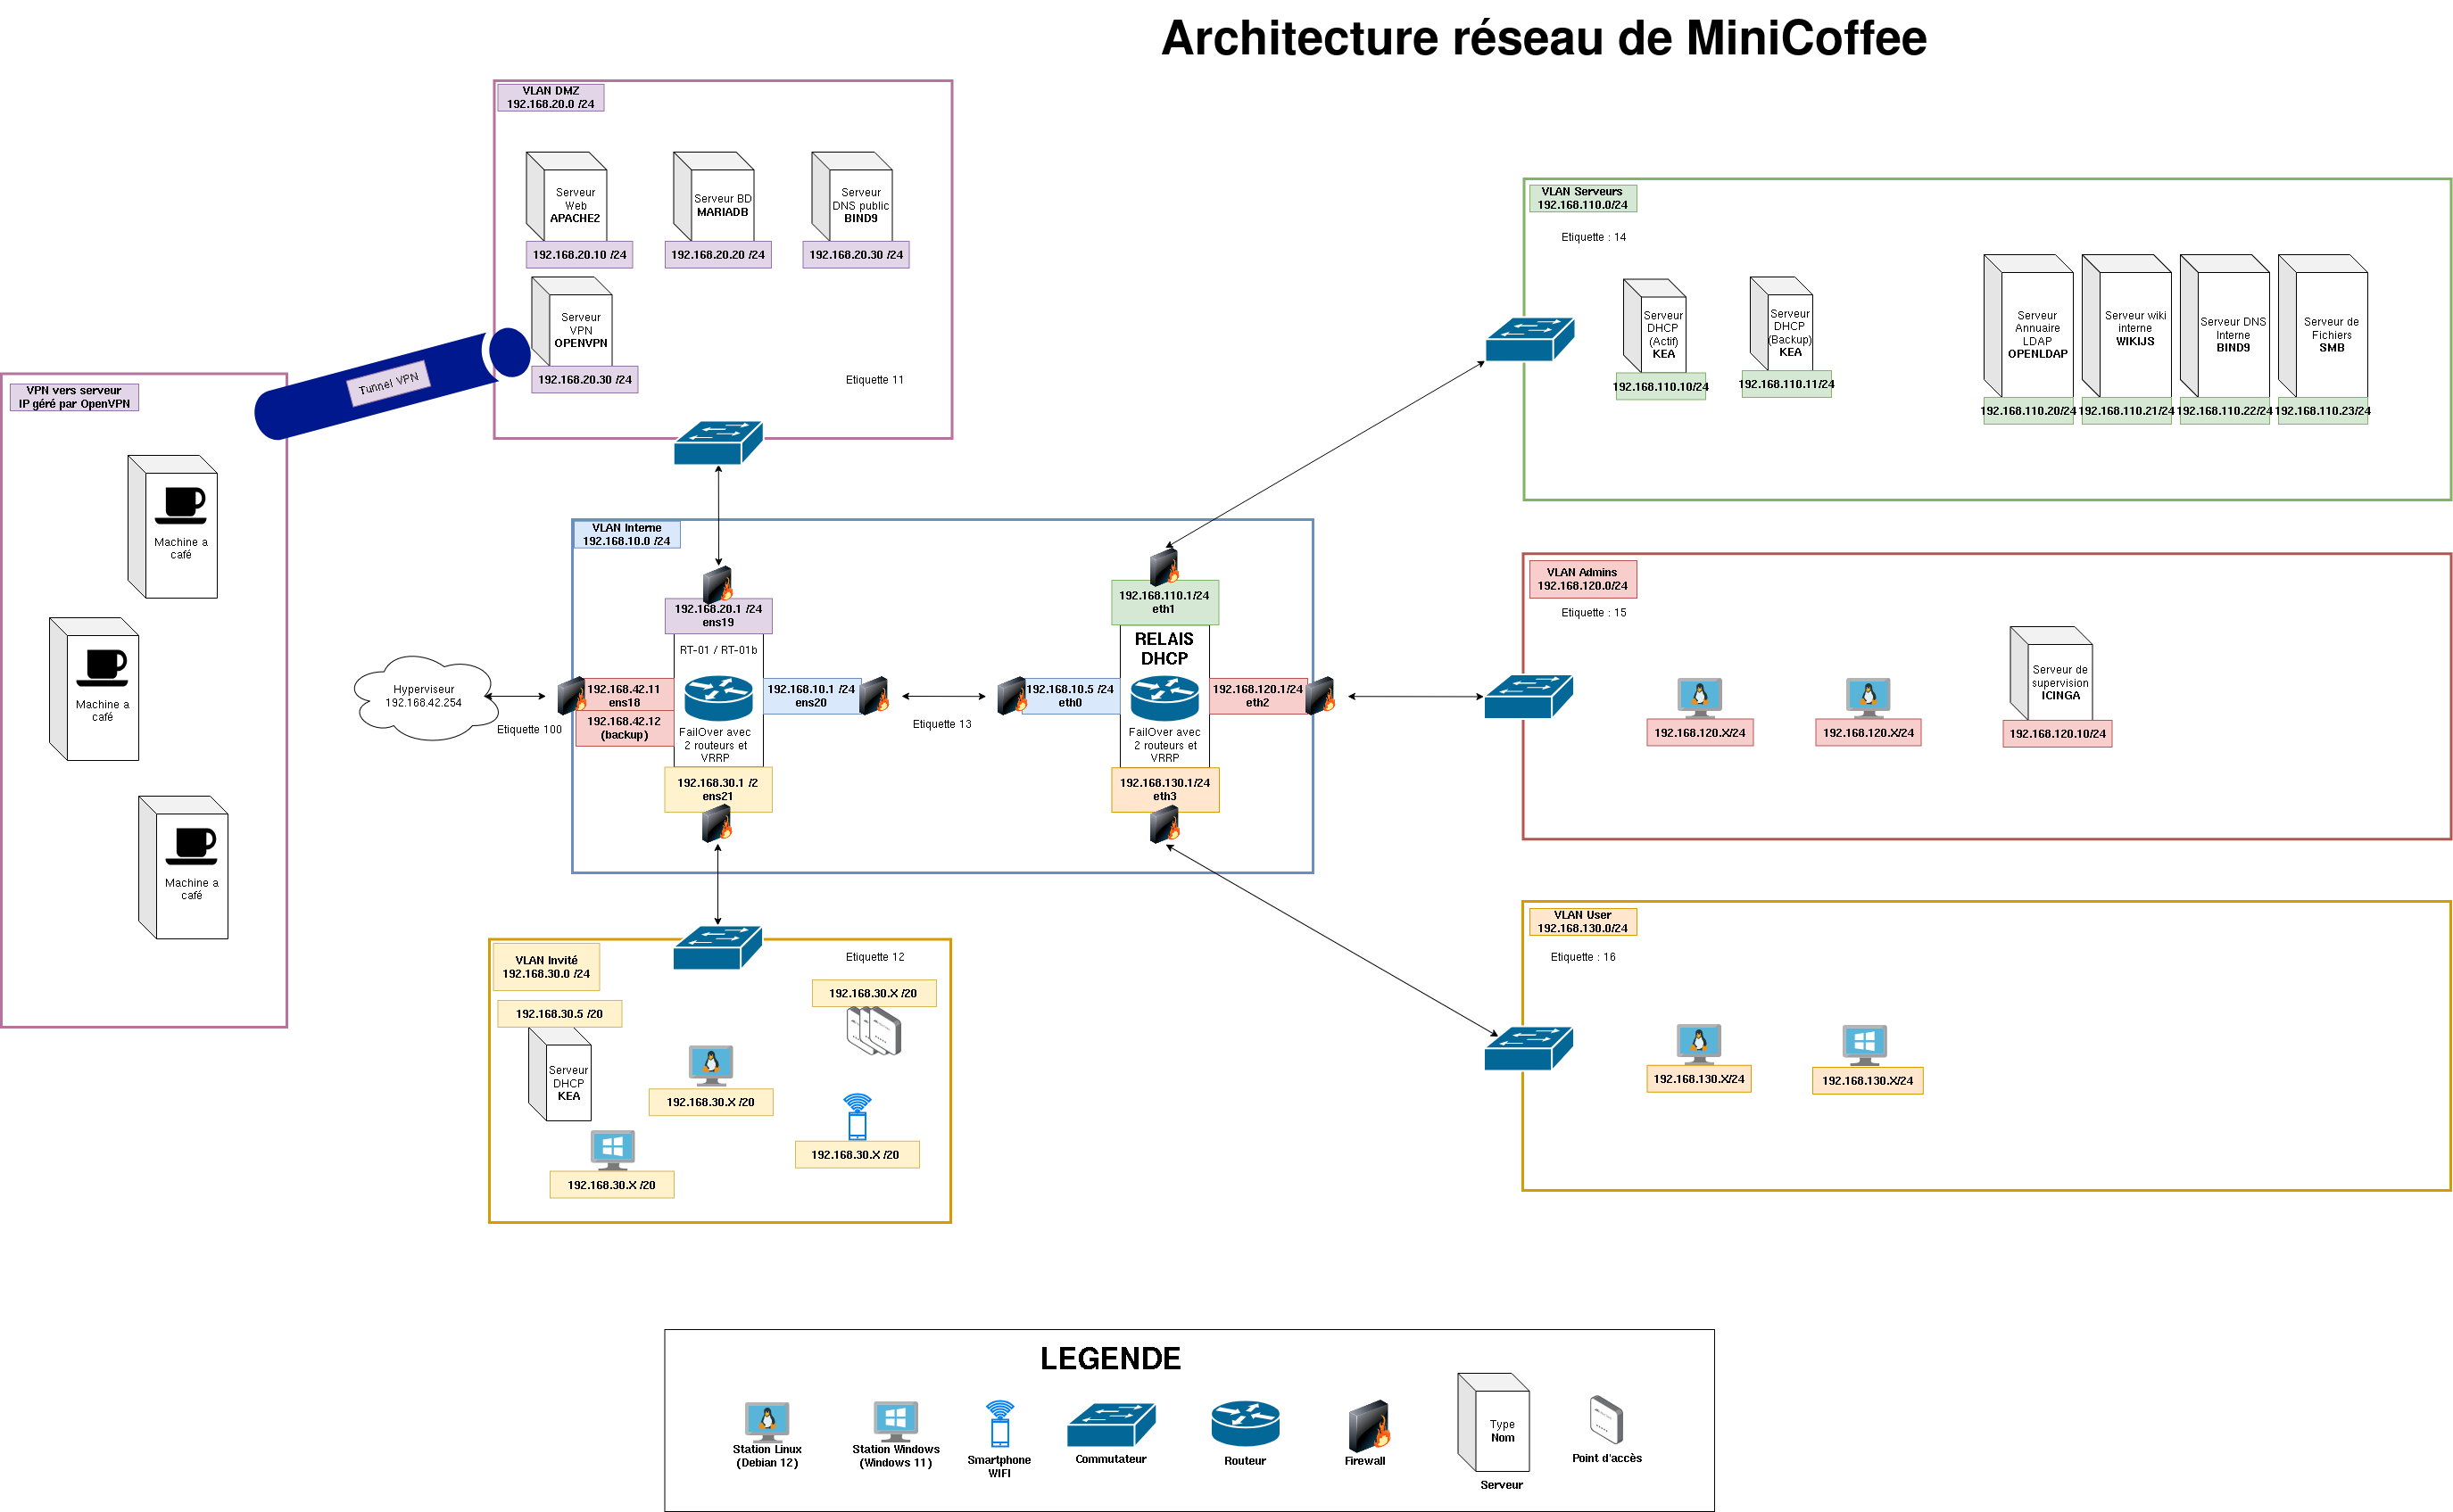
\includegraphics[width=1.2\textwidth, trim=0 0 0 2.3cm, clip]{../assets/Architecture.drawio.png}
    \caption{Architecture réseau de MiniCoffee}
\end{figure}

\clearpage

\section{Ressources Matérielles utilisées}
Actuellement, notre infrastructure réseau comprend un total de 9 machines actives, chacune jouant un rôle spécifique dans notre environnement.
\\

En ce qui concerne le stockage, nous allouons entre 3 et 5 Go d’espace disque par machine, en fonction de leurs besoins en ressources et des tâches qu’elles doivent accomplir. Plus précisément :
\begin{itemize}
    \item Les machines nécessitant le moins de ressources se voient attribuer 3 Go de stockage, ce qui est suffisant pour assurer leur bon fonctionnement sans surconsommation d’espace.
    \item Les machines les plus sollicitées, qui traitent des volumes de données plus importants ou exécutent des processus plus intensifs, bénéficient quant à elles de 5 Go de stockage afin de garantir des performances optimales.
\end{itemize}

En termes de mémoire vive (RAM), chaque machine de notre réseau dispose actuellement de 1 Go. Cette allocation permet de répondre aux besoins de nos applications tout en maintenant un bon équilibre entre performance et consommation de ressources.
\\

Nous surveillons régulièrement l’utilisation de la RAM et du stockage afin d’optimiser notre infrastructure si nécessaire et d’anticiper toute montée en charge.

\end{document}